\documentclass[aspectratio=169,11pt]{beamer}
\usetheme{default}
\usepackage[T1]{fontenc}
\usepackage{helvet}\renewcommand{\familydefault}{\sfdefault}
\usepackage{booktabs}
\usepackage{graphicx}
\usepackage{xcolor}
% Auto-generated by experiments/make_numbers.py. Do not edit by hand.
\newcommand{\BestDeepTEightFps}{0.910}
\newcommand{\BestDeepTEightFzero}{0.629}
\newcommand{\BestDeepTEightGain}{1.135}
\newcommand{\BestDeepTEightIllegal}{0}
\newcommand{\BestDeepTEightKeep}{0.615}
\newcommand{\BestDeepTEightPolicy}{safe}
\newcommand{\BestDeepTEightTargets}{q0,q3,q4}
\newcommand{\BestDeepTFourFps}{0.910}
\newcommand{\BestDeepTFourFzero}{0.632}
\newcommand{\BestDeepTFourGain}{1.130}
\newcommand{\BestDeepTFourIllegal}{0}
\newcommand{\BestDeepTFourKeep}{0.615}
\newcommand{\BestDeepTFourPolicy}{safe}
\newcommand{\BestDeepTFourTargets}{q0,q3,q4}
\newcommand{\BestDeepTOneFps}{0.909}
\newcommand{\BestDeepTOneFzero}{0.637}
\newcommand{\BestDeepTOneGain}{1.119}
\newcommand{\BestDeepTOneIllegal}{0}
\newcommand{\BestDeepTOneKeep}{0.615}
\newcommand{\BestDeepTOnePolicy}{safe}
\newcommand{\BestDeepTOneTargets}{q0,q3,q4}
\newcommand{\BestDeepTSixteenFps}{0.863}
\newcommand{\BestDeepTSixteenFzero}{0.629}
\newcommand{\BestDeepTSixteenGain}{1.120}
\newcommand{\BestDeepTSixteenIllegal}{13}
\newcommand{\BestDeepTSixteenKeep}{0.666}
\newcommand{\BestDeepTSixteenPolicy}{safe}
\newcommand{\BestDeepTSixteenTargets}{q2,q3}
\newcommand{\BestDeepTTwoFps}{0.910}
\newcommand{\BestDeepTTwoFzero}{0.634}
\newcommand{\BestDeepTTwoGain}{1.126}
\newcommand{\BestDeepTTwoIllegal}{0}
\newcommand{\BestDeepTTwoKeep}{0.615}
\newcommand{\BestDeepTTwoPolicy}{safe}
\newcommand{\BestDeepTTwoTargets}{q0,q3,q4}
\newcommand{\BestDeepTZeroFps}{0.910}
\newcommand{\BestDeepTZeroFzero}{0.637}
\newcommand{\BestDeepTZeroGain}{1.119}
\newcommand{\BestDeepTZeroIllegal}{0}
\newcommand{\BestDeepTZeroKeep}{0.615}
\newcommand{\BestDeepTZeroPolicy}{none}
\newcommand{\BestDeepTZeroTargets}{q0,q3,q5}
\newcommand{\BestMediumTEightFps}{0.894}
\newcommand{\BestMediumTEightFzero}{0.722}
\newcommand{\BestMediumTEightGain}{1.073}
\newcommand{\BestMediumTEightIllegal}{0}
\newcommand{\BestMediumTEightKeep}{0.750}
\newcommand{\BestMediumTEightPolicy}{safe}
\newcommand{\BestMediumTEightTargets}{q0,q3}
\newcommand{\BestMediumTFourFps}{0.894}
\newcommand{\BestMediumTFourFzero}{0.722}
\newcommand{\BestMediumTFourGain}{1.072}
\newcommand{\BestMediumTFourIllegal}{0}
\newcommand{\BestMediumTFourKeep}{0.750}
\newcommand{\BestMediumTFourPolicy}{safe}
\newcommand{\BestMediumTFourTargets}{q0,q3}
\newcommand{\BestMediumTOneFps}{0.896}
\newcommand{\BestMediumTOneFzero}{0.722}
\newcommand{\BestMediumTOneGain}{1.074}
\newcommand{\BestMediumTOneIllegal}{0}
\newcommand{\BestMediumTOneKeep}{0.750}
\newcommand{\BestMediumTOnePolicy}{safe}
\newcommand{\BestMediumTOneTargets}{q0,q3}
\newcommand{\BestMediumTSixteenFps}{0.895}
\newcommand{\BestMediumTSixteenFzero}{0.722}
\newcommand{\BestMediumTSixteenGain}{1.074}
\newcommand{\BestMediumTSixteenIllegal}{10}
\newcommand{\BestMediumTSixteenKeep}{0.750}
\newcommand{\BestMediumTSixteenPolicy}{safe}
\newcommand{\BestMediumTSixteenTargets}{q0,q3}
\newcommand{\BestMediumTTwoFps}{0.896}
\newcommand{\BestMediumTTwoFzero}{0.722}
\newcommand{\BestMediumTTwoGain}{1.074}
\newcommand{\BestMediumTTwoIllegal}{0}
\newcommand{\BestMediumTTwoKeep}{0.750}
\newcommand{\BestMediumTTwoPolicy}{safe}
\newcommand{\BestMediumTTwoTargets}{q0,q3}
\newcommand{\BestMediumTZeroFps}{0.896}
\newcommand{\BestMediumTZeroFzero}{0.722}
\newcommand{\BestMediumTZeroGain}{1.074}
\newcommand{\BestMediumTZeroIllegal}{0}
\newcommand{\BestMediumTZeroKeep}{0.750}
\newcommand{\BestMediumTZeroPolicy}{none}
\newcommand{\BestMediumTZeroTargets}{q0,q3}
\newcommand{\BestShallowTEightFps}{0.911}
\newcommand{\BestShallowTEightFzero}{0.831}
\newcommand{\BestShallowTEightGain}{1.011}
\newcommand{\BestShallowTEightIllegal}{0}
\newcommand{\BestShallowTEightKeep}{0.851}
\newcommand{\BestShallowTEightPolicy}{safe}
\newcommand{\BestShallowTEightTargets}{q0,q4}
\newcommand{\BestShallowTFourFps}{0.914}
\newcommand{\BestShallowTFourFzero}{0.832}
\newcommand{\BestShallowTFourGain}{1.013}
\newcommand{\BestShallowTFourIllegal}{0}
\newcommand{\BestShallowTFourKeep}{0.851}
\newcommand{\BestShallowTFourPolicy}{safe}
\newcommand{\BestShallowTFourTargets}{q0,q4}
\newcommand{\BestShallowTOneFps}{0.914}
\newcommand{\BestShallowTOneFzero}{0.828}
\newcommand{\BestShallowTOneGain}{1.018}
\newcommand{\BestShallowTOneIllegal}{0}
\newcommand{\BestShallowTOneKeep}{0.851}
\newcommand{\BestShallowTOnePolicy}{safe}
\newcommand{\BestShallowTOneTargets}{q0,q4}
\newcommand{\BestShallowTSixteenFps}{0.911}
\newcommand{\BestShallowTSixteenFzero}{0.833}
\newcommand{\BestShallowTSixteenGain}{1.009}
\newcommand{\BestShallowTSixteenIllegal}{2}
\newcommand{\BestShallowTSixteenKeep}{0.851}
\newcommand{\BestShallowTSixteenPolicy}{safe}
\newcommand{\BestShallowTSixteenTargets}{q0,q4}
\newcommand{\BestShallowTTwoFps}{0.914}
\newcommand{\BestShallowTTwoFzero}{0.828}
\newcommand{\BestShallowTTwoGain}{1.018}
\newcommand{\BestShallowTTwoIllegal}{0}
\newcommand{\BestShallowTTwoKeep}{0.851}
\newcommand{\BestShallowTTwoPolicy}{safe}
\newcommand{\BestShallowTTwoTargets}{q0,q4}
\newcommand{\BestShallowTZeroFps}{0.914}
\newcommand{\BestShallowTZeroFzero}{0.828}
\newcommand{\BestShallowTZeroGain}{1.018}
\newcommand{\BestShallowTZeroIllegal}{0}
\newcommand{\BestShallowTZeroKeep}{0.851}
\newcommand{\BestShallowTZeroPolicy}{none}
\newcommand{\BestShallowTZeroTargets}{q0,q4}
\newcommand{\BestTableRows}{6 & 0 & $q_{0,4}$, Clifford & 0.828 & 0.914 (0.851) & 1.018 \\ 6 & 1 & $q_{0,4}$, safe & 0.828 & 0.914 (0.851) & 1.018 \\ 6 & 2 & $q_{0,4}$, safe & 0.828 & 0.914 (0.851) & 1.018 \\ 6 & 4 & $q_{0,4}$, safe & 0.832 & 0.914 (0.851) & 1.013 \\ 6 & 8 & $q_{0,4}$, safe & 0.831 & 0.911 (0.851) & 1.011 \\ 6 & 16 & $q_{0,4}$, safe & 0.833 & 0.911 (0.851) & 1.009 \\ 12 & 0 & $q_{0,3}$, Clifford & 0.722 & 0.896 (0.750) & 1.074 \\ 12 & 1 & $q_{0,3}$, safe & 0.722 & 0.896 (0.750) & 1.074 \\ 12 & 2 & $q_{0,3}$, safe & 0.722 & 0.896 (0.750) & 1.074 \\ 12 & 4 & $q_{0,3}$, safe & 0.722 & 0.894 (0.750) & 1.072 \\ 12 & 8 & $q_{0,3}$, safe & 0.722 & 0.894 (0.750) & 1.073 \\ 12 & 16 & $q_{0,3}$, safe & 0.722 & 0.895 (0.750) & 1.074 \\ 18 & 0 & $q_{0,3,5}$, Clifford & 0.637 & 0.910 (0.615) & 1.119 \\ 18 & 1 & $q_{0,3,4}$, safe & 0.637 & 0.909 (0.615) & 1.119 \\ 18 & 2 & $q_{0,3,4}$, safe & 0.634 & 0.910 (0.615) & 1.126 \\ 18 & 4 & $q_{0,3,4}$, safe & 0.632 & 0.910 (0.615) & 1.130 \\ 18 & 8 & $q_{0,3,4}$, safe & 0.629 & 0.910 (0.615) & 1.135 \\ 18 & 16 & $q_{2,3}$, safe & 0.629 & 0.863 (0.666) & 1.120}
\newcommand{\CapDeepFour}{14.3}
\newcommand{\CapDeepOne}{49.6}
\newcommand{\CapDeepSix}{7.4}
\newcommand{\CapDeepTwo}{29.4}
\newcommand{\CapDeepZero}{90.0}
\newcommand{\CapFracDeepFour}{16\%}
\newcommand{\CapFracDeepOne}{55\%}
\newcommand{\CapFracDeepSix}{8\%}
\newcommand{\CapFracDeepTwo}{33\%}
\newcommand{\CapFracDeepZero}{100\%}
\newcommand{\CapFracHugeFour}{14\%}
\newcommand{\CapFracHugeOne}{53\%}
\newcommand{\CapFracHugeSix}{10\%}
\newcommand{\CapFracHugeTwo}{31\%}
\newcommand{\CapFracHugeZero}{100\%}
\newcommand{\CapFracMediumFour}{33\%}
\newcommand{\CapFracMediumOne}{69\%}
\newcommand{\CapFracMediumSix}{27\%}
\newcommand{\CapFracMediumTwo}{51\%}
\newcommand{\CapFracMediumZero}{100\%}
\newcommand{\CapFracShallowFour}{62\%}
\newcommand{\CapFracShallowOne}{87\%}
\newcommand{\CapFracShallowSix}{50\%}
\newcommand{\CapFracShallowTwo}{76\%}
\newcommand{\CapFracShallowZero}{100\%}
\newcommand{\CapHugeFour}{16.9}
\newcommand{\CapHugeOne}{64.0}
\newcommand{\CapHugeSix}{11.8}
\newcommand{\CapHugeTwo}{37.2}
\newcommand{\CapHugeZero}{120.0}
\newcommand{\CapMediumFour}{19.5}
\newcommand{\CapMediumOne}{41.3}
\newcommand{\CapMediumSix}{16.0}
\newcommand{\CapMediumTwo}{30.4}
\newcommand{\CapMediumZero}{60.0}
\newcommand{\CapMinDeepFour}{6}
\newcommand{\CapMinDeepOne}{38}
\newcommand{\CapMinDeepSix}{6}
\newcommand{\CapMinDeepTwo}{17}
\newcommand{\CapMinDeepZero}{90}
\newcommand{\CapMinHugeFour}{4}
\newcommand{\CapMinHugeOne}{50}
\newcommand{\CapMinHugeSix}{7}
\newcommand{\CapMinHugeTwo}{24}
\newcommand{\CapMinHugeZero}{120}
\newcommand{\CapMinMediumFour}{7}
\newcommand{\CapMinMediumOne}{30}
\newcommand{\CapMinMediumSix}{10}
\newcommand{\CapMinMediumTwo}{14}
\newcommand{\CapMinMediumZero}{60}
\newcommand{\CapMinShallowFour}{11}
\newcommand{\CapMinShallowOne}{19}
\newcommand{\CapMinShallowSix}{12}
\newcommand{\CapMinShallowTwo}{16}
\newcommand{\CapMinShallowZero}{30}
\newcommand{\CapShallowFour}{18.5}
\newcommand{\CapShallowOne}{26.1}
\newcommand{\CapShallowSix}{15.0}
\newcommand{\CapShallowTwo}{22.7}
\newcommand{\CapShallowZero}{30.0}
\newcommand{\CapTotalDeep}{90}
\newcommand{\CapTotalHuge}{120}
\newcommand{\CapTotalMedium}{60}
\newcommand{\CapTotalShallow}{30}
\newcommand{\EfiveGainDeepHigh}{1.177}
\newcommand{\EfiveGainDeepLow}{1.009}
\newcommand{\EfiveGainDeepMid}{1.088}
\newcommand{\EfiveGainMediumHigh}{1.045}
\newcommand{\EfiveGainMediumLow}{1.004}
\newcommand{\EfiveGainMediumMid}{1.030}
\newcommand{\EfiveGainShallowHigh}{0.906}
\newcommand{\EfiveGainShallowLow}{0.997}
\newcommand{\EfiveGainShallowMid}{0.973}
\newcommand{\EoneFpsDeep}{0.886}
\newcommand{\EoneFpsMedium}{0.883}
\newcommand{\EoneFpsShallow}{0.828}
\newcommand{\EoneFpsSixDeep}{0.939}
\newcommand{\EoneFpsSixMedium}{0.921}
\newcommand{\EoneFpsSixShallow}{0.912}
\newcommand{\EoneFzeroDeep}{0.629}
\newcommand{\EoneFzeroMedium}{0.720}
\newcommand{\EoneFzeroShallow}{0.828}
\newcommand{\EoneGainDeep}{1.103}
\newcommand{\EoneGainMedium}{1.037}
\newcommand{\EoneGainOneDeep}{1.067}
\newcommand{\EoneGainOneMedium}{1.021}
\newcommand{\EoneGainOneShallow}{0.993}
\newcommand{\EoneGainShallow}{1.000}
\newcommand{\EoneGammaZeroDeep}{1.866}
\newcommand{\EoneGammaZeroMedium}{1.721}
\newcommand{\EoneGammaZeroShallow}{1.350}
\newcommand{\EoneKDeep}{3}
\newcommand{\EoneKMedium}{3}
\newcommand{\EoneKShallow}{0}
\newcommand{\EoneKeepDeep}{0.612}
\newcommand{\EoneKeepMedium}{0.716}
\newcommand{\EoneKeepShallow}{1.000}
\newcommand{\EoneKeepSixDeep}{0.499}
\newcommand{\EoneKeepSixMedium}{0.599}
\newcommand{\EoneKeepSixShallow}{0.723}
\newcommand{\EsevenFpsHighTSixteen}{0.837}
\newcommand{\EsevenFpsHighTZero}{0.890}
\newcommand{\EsevenFpsZeroTSixteen}{0.891}
\newcommand{\EsevenFpsZeroTZero}{0.890}
\newcommand{\EsevenFzeroHighTSixteen}{0.640}
\newcommand{\EsevenFzeroHighTZero}{0.721}
\newcommand{\EsevenFzeroZeroTSixteen}{0.720}
\newcommand{\EsevenFzeroZeroTZero}{0.721}
\newcommand{\EtwoBlindFDeepTFour}{0.507}
\newcommand{\EtwoBlindFDeepTSixteen}{0.158}
\newcommand{\EtwoBlindFMediumTFour}{0.543}
\newcommand{\EtwoBlindFMediumTSixteen}{0.260}
\newcommand{\EtwoBlindKDeepTFour}{0.388}
\newcommand{\EtwoBlindKDeepTSixteen}{0.174}
\newcommand{\EtwoBlindKMediumTFour}{0.472}
\newcommand{\EtwoBlindKMediumTSixteen}{0.248}
\newcommand{\EtwoBrokenFourDeep}{2.4}
\newcommand{\EtwoBrokenFourMedium}{1.8}
\newcommand{\EtwoCliffDeep}{0.896}
\newcommand{\EtwoCliffKeepDeep}{0.606}
\newcommand{\EtwoCliffKeepMedium}{0.710}
\newcommand{\EtwoCliffMedium}{0.892}
\newcommand{\EtwoNoneFDeepTFour}{0.627}
\newcommand{\EtwoNoneFDeepTSixteen}{0.628}
\newcommand{\EtwoNoneFMediumTFour}{0.719}
\newcommand{\EtwoNoneFMediumTSixteen}{0.719}
\newcommand{\EtwoNoneFzeroTSixteenDeep}{0.628}
\newcommand{\EtwoNoneFzeroTSixteenMedium}{0.719}
\newcommand{\EtwoNoneFzeroTZeroDeep}{0.629}
\newcommand{\EtwoNoneFzeroTZeroMedium}{0.720}
\newcommand{\EtwoNoneKDeepTFour}{1.000}
\newcommand{\EtwoNoneKDeepTSixteen}{1.000}
\newcommand{\EtwoNoneKMediumTFour}{1.000}
\newcommand{\EtwoNoneKMediumTSixteen}{1.000}
\newcommand{\EtwoRetireFDeepTFour}{0.282}
\newcommand{\EtwoRetireFDeepTSixteen}{0.102}
\newcommand{\EtwoRetireFMediumTFour}{0.386}
\newcommand{\EtwoRetireFMediumTSixteen}{0.176}
\newcommand{\EtwoRetireKDeepTFour}{0.875}
\newcommand{\EtwoRetireKDeepTSixteen}{1.000}
\newcommand{\EtwoRetireKMediumTFour}{0.889}
\newcommand{\EtwoRetireKMediumTSixteen}{0.970}
\newcommand{\EtwoSafeDrift}{0.004}
\newcommand{\EtwoSafeFDeepTFour}{0.896}
\newcommand{\EtwoSafeFDeepTSixteen}{0.892}
\newcommand{\EtwoSafeFMediumTFour}{0.891}
\newcommand{\EtwoSafeFMediumTSixteen}{0.889}
\newcommand{\EtwoSafeKDeepTFour}{0.606}
\newcommand{\EtwoSafeKDeepTSixteen}{0.604}
\newcommand{\EtwoSafeKMediumTFour}{0.710}
\newcommand{\EtwoSafeKMediumTSixteen}{0.715}
\newcommand{\FezFzeroDeep}{0.789}
\newcommand{\FezFzeroMedium}{0.835}
\newcommand{\FezFzeroShallow}{0.891}
\newcommand{\FezGainDeep}{1.060}
\newcommand{\FezGainMedium}{1.045}
\newcommand{\FezGainShallow}{1.015}
\newcommand{\FezKDeep}{3}
\newcommand{\FezKMedium}{2}
\newcommand{\FezKShallow}{2}
\newcommand{\FzeroDeep}{0.637}
\newcommand{\FzeroMedium}{0.722}
\newcommand{\FzeroShallow}{0.828}
\newcommand{\GridMinutes}{53}
\newcommand{\HzeroDeep}{1.000}
\newcommand{\LocMaxDeep}{1.106}
\newcommand{\LocMaxShallow}{1.018}
\newcommand{\LocMinDeep}{1.062}
\newcommand{\LocMinShallow}{0.976}
\newcommand{\NumIllegal}{25}
\newcommand{\NumMoves}{5{,}412}
\newcommand{\NumMovesPerProfile}{2{,}706}
\newcommand{\ProFez}{0.0088}
\newcommand{\PtwoFez}{0.0048}
\newcommand{\ValHdiff}{0.011}
\newcommand{\ValKeepSigma}{1.4}
\newcommand{\ValStabDiff}{3e-15}

\definecolor{ink}{HTML}{111827}
\definecolor{acc}{HTML}{2563EB}
\definecolor{teal}{HTML}{0F9F8F}
\definecolor{magic}{HTML}{C98A00}
\definecolor{bad}{HTML}{D6264B}
\setbeamercolor{frametitle}{fg=ink}
\setbeamercolor{normal text}{fg=ink}
\setbeamercolor{structure}{fg=acc}
\setbeamerfont{frametitle}{size=\Large,series=\bfseries}
\setbeamertemplate{navigation symbols}{}
\setbeamertemplate{footline}{\hfill\scriptsize\color{gray}Spacetime Sentinels \quad \insertframenumber\hspace{1em}\vspace{0.6em}}
\graphicspath{{../report/figures/}}
\newcommand{\hl}[1]{\textcolor{acc}{\textbf{#1}}}

\title{Spacetime Sentinels}
\subtitle{A game of low-overhead error detection with spacetime codes,\\ scored entirely with Qiskit}
\author{Sumit Tapas Chongder \and Aditya Kumar}
\institute{Department of CSE and Department of Physics, IIT Jodhpur\\[2pt]\small Qiskit Fall Fest 2026 Hackathon, Advanced track}
\date{}

\begin{document}

\begin{frame}
\titlepage
\end{frame}

\begin{frame}{The question}
\begin{itemize}\setlength\itemsep{8pt}
  \item How do we get students to \hl{feel} why fault tolerance is hard?
  \item Our brief: a game built on \hl{error detection with spacetime codes} (\texttt{qiskit-paulice}).
  \item Rules must be the physics. Scores must come from Qiskit, never from hand-set values.
\end{itemize}
\vspace{10pt}
\begin{columns}[T]
\column{0.32\textwidth}\textbf{\textcolor{teal}{Detection (us)}}\\\small flag what the checks see, discard those shots. Nothing is repaired.
\column{0.32\textwidth}\textbf{Mitigation}\\\small fix the \emph{estimate} afterwards (ZNE, PEC, twirling, readout).
\column{0.32\textwidth}\textbf{Correction}\\\small logical qubits, repeated stabilizers, a decoder that undoes errors.
\end{columns}
\end{frame}

\begin{frame}{A spacetime check in one picture}
\begin{columns}[c]
\column{0.5\textwidth}
\begin{itemize}\setlength\itemsep{6pt}
  \item One ancilla, one target qubit.
  \item Controlled $X$, $Y$ or $Z$ at a few moments in time.
  \item Syndrome = ancilla bit $\oplus$ parity of some outputs. Deterministic if nothing went wrong.
  \item A fault is caught if it anticommutes with the check's \hl{flow} at that point.
\end{itemize}
\column{0.5\textwidth}
\textbf{The catch: $T$ gates}\\[4pt]
$TZT^\dagger = Z$ \quad but \quad $TXT^\dagger=\frac{X+Y}{\sqrt2}$\\[6pt]
A $T$ on a wire where some check acts as $X/Y$ \textcolor{bad}{breaks} that check.\\[6pt]
On IBM hardware $T$ is a virtual $R_Z$: \hl{free in noise}, not free for the code.
\end{columns}
\end{frame}

\begin{frame}{The game}
\centering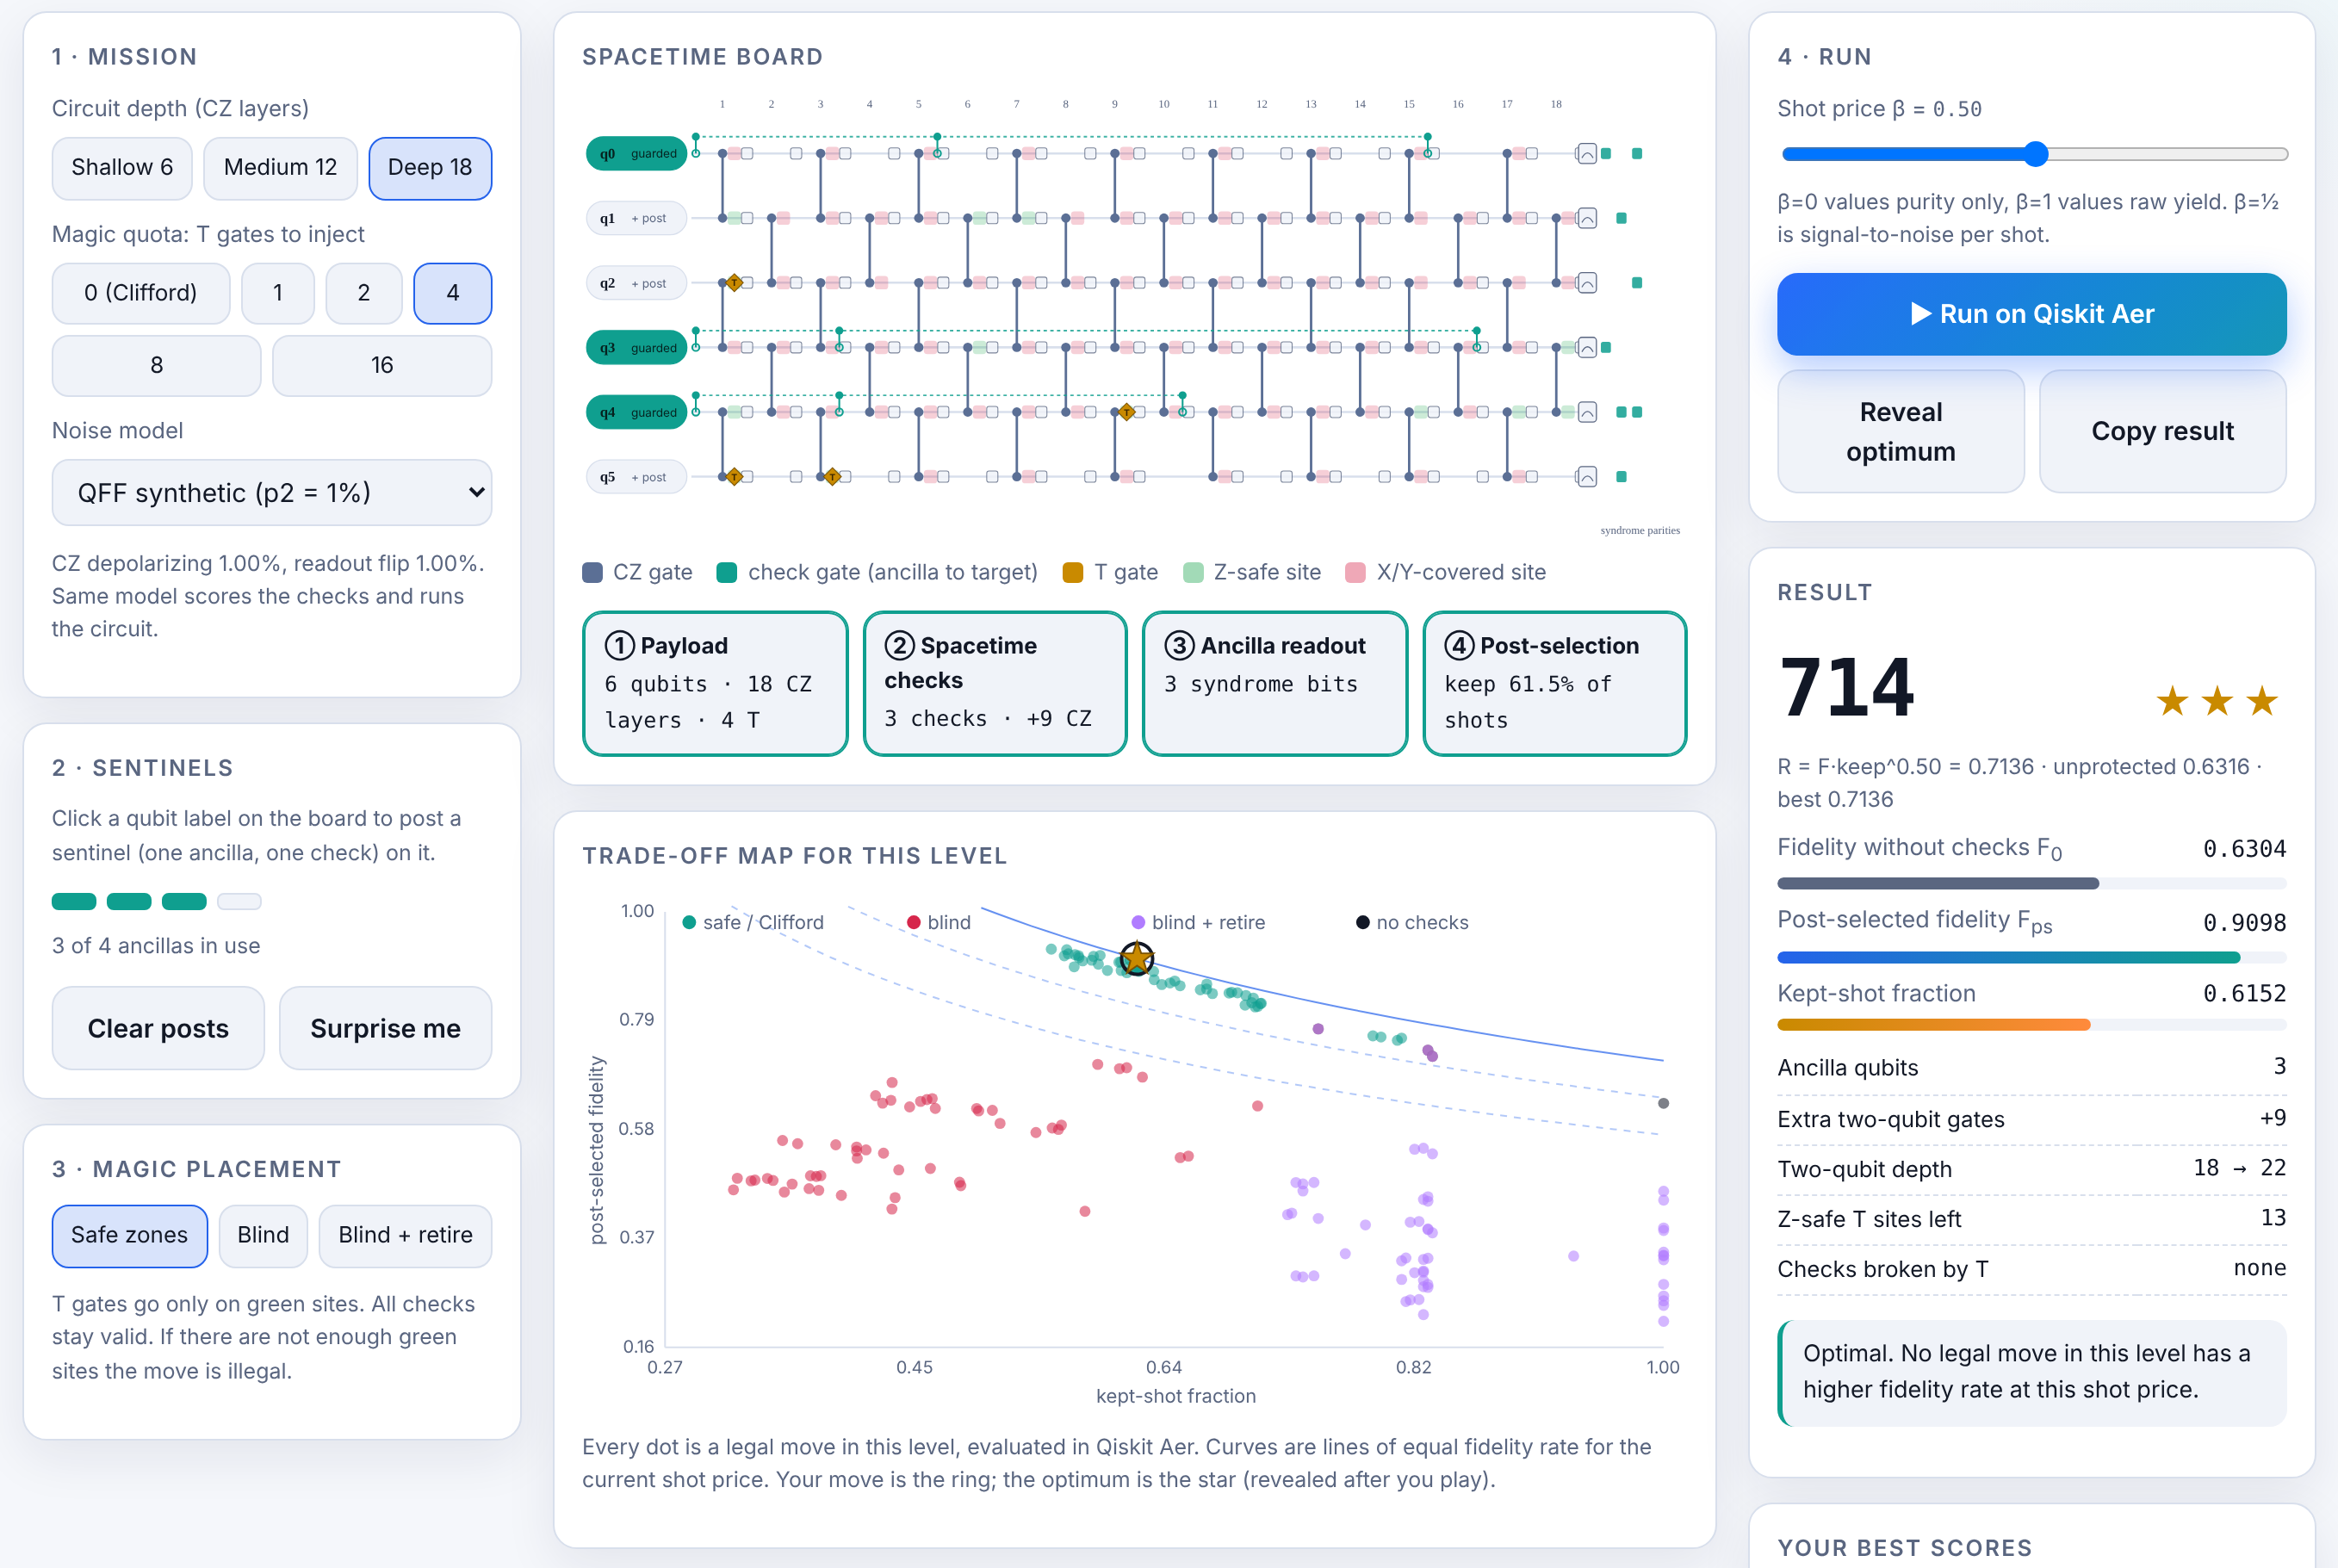
\includegraphics[height=0.86\textheight]{board.png}
\end{frame}

\begin{frame}{Every rule is a physics decision}
\small
\begin{tabular}{p{0.3\textwidth}p{0.6\textwidth}}
\toprule
Rule & Physics (and the Qiskit call behind it)\\
\midrule
Post a sentinel (budget 4) & one ancilla + one spacetime check, \texttt{add\_pauli\_checks}\\
Green / red sites & every check acts as $I/Z$ there or not, \texttt{uncovered\_paulis}\\
Magic quota & number of $T$ gates in the payload\\
Safe / Blind / Retire & doping policy; broken checks detected by noiseless statevector\\
Run & payload $\to$ checks $\to$ ancilla readout $\to$ post-selection, Aer density matrix\\
Score $1000\,F_{ps}\kappa^{\beta}$ & fidelity rate; $\beta=\tfrac12$ is SNR per $\sqrt{\text{shot}}$\\
\bottomrule
\end{tabular}
\vspace{6pt}
\par\NumMoves{} legal moves, every one evaluated exactly with Qiskit Aer.
\end{frame}

\begin{frame}{Why $R=F_{ps}\sqrt{\kappa}$?}
\begin{itemize}\setlength\itemsep{8pt}
  \item Residual error damps an observable by $F_{ps}$; we keep $\kappa N$ of $N$ shots.
  \item Rescaled estimate has error $\sim \sigma/(F_{ps}\sqrt{\kappa N})$.
  \item Shots needed $\propto 1/(F_{ps}^2\kappa)=R_{1/2}^{-2}$: the overhead of \hl{detection then mitigation}.
  \item No checks: $R=F_0$. Gain $G=R/F_0>1$ means the sentinels paid for themselves.
\end{itemize}
\end{frame}

\begin{frame}{Finding 1: checks only pay above a break-even depth}
\centering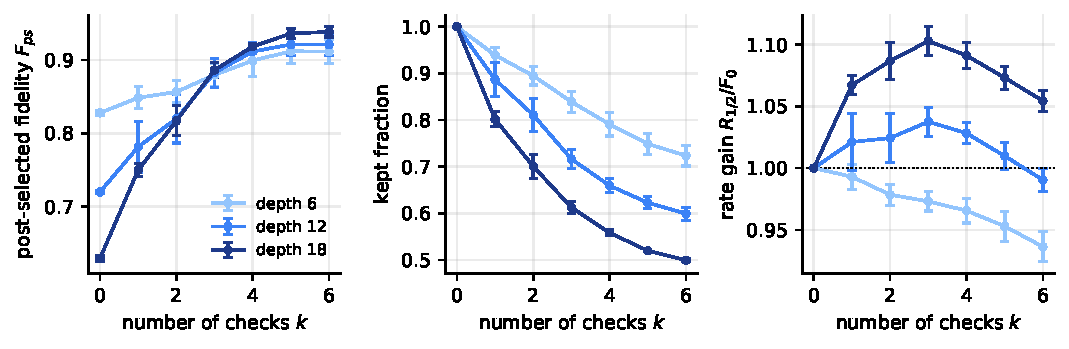
\includegraphics[width=0.95\textwidth]{fig_check_count.pdf}\\
\small Depth 6: every check lowers $R$ (one check: $G=\EoneGainOneShallow$). Best gain at depth 12: \EoneGainMedium{} ($k=\EoneKMedium$); depth 18: \EoneGainDeep{} ($k=\EoneKDeep$). Five random payloads.
\end{frame}

\begin{frame}{Finding 2: $T$ count against check placement}
\centering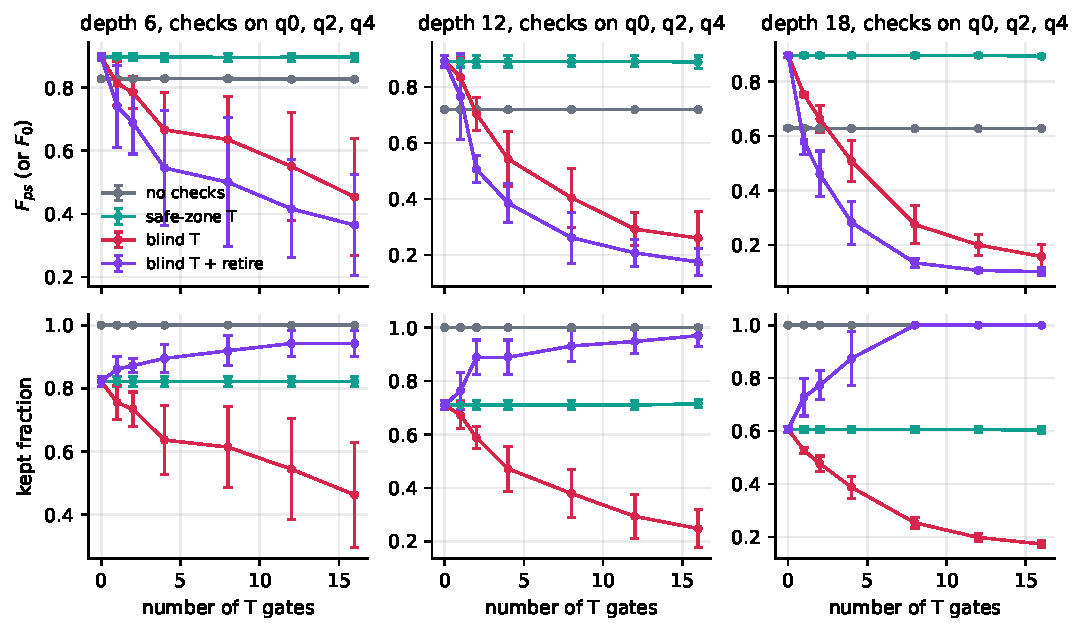
\includegraphics[height=0.72\textheight]{fig_t_count.pdf}\\
\small Depth 18, 16 $T$ gates: safe zones $F_{ps}=\EtwoSafeFDeepTSixteen$, blind \EtwoBlindFDeepTSixteen, blind + retire \EtwoRetireFDeepTSixteen, no checks \EtwoNoneFDeepTSixteen.
\end{frame}

\begin{frame}{Finding 3: protection and magic compete for spacetime}
\begin{columns}[c]
\column{0.58\textwidth}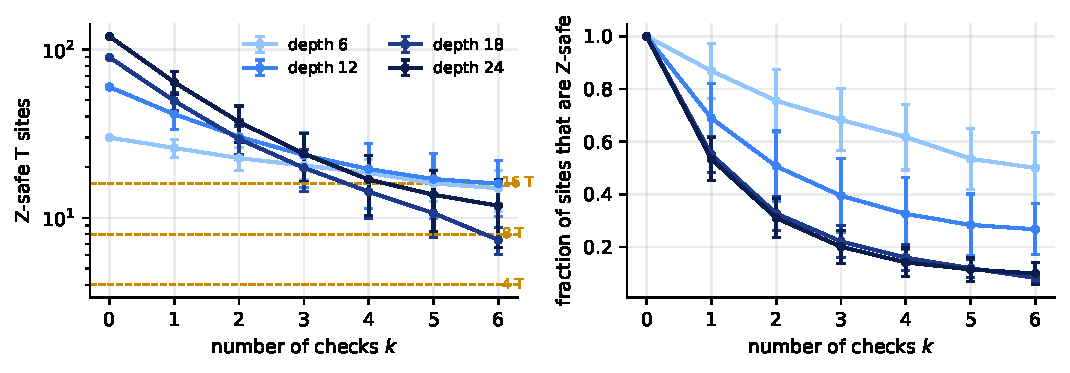
\includegraphics[width=\textwidth]{fig_capacity.pdf}
\column{0.42\textwidth}\small
Z-safe $T$ sites at depth 18:\\
0 checks: \CapDeepZero{} of \CapTotalDeep\\
2 checks: \CapDeepTwo\\
4 checks: \CapDeepFour\\
6 checks: \CapDeepSix\\[6pt]
Every check you add removes places where magic can go. \NumIllegal{} moves in the game are illegal for exactly this reason.
\end{columns}
\end{frame}

\begin{frame}{Finding 4: a broken check is worse than no check}
\begin{itemize}\setlength\itemsep{8pt}
  \item Blind $T$ placement broke on average \EtwoBrokenFourDeep{} of 3 checks (depth 18, 4 $T$).
  \item Listening to a broken check throws away good shots: it fires on perfect runs.
  \item \hl{Ignoring it does not help}: its gates still entangle the ancilla with a non-stabilizer operator, a partial measurement that destroys coherence.
  \item Depth 18, 4 $T$: blind + retire $F_{ps}=\EtwoRetireFDeepTFour$ vs.\ no checks $F_0=\EtwoNoneFDeepTFour$.
\end{itemize}
\end{frame}

\begin{frame}{The best trade-off and why it wins}
\centering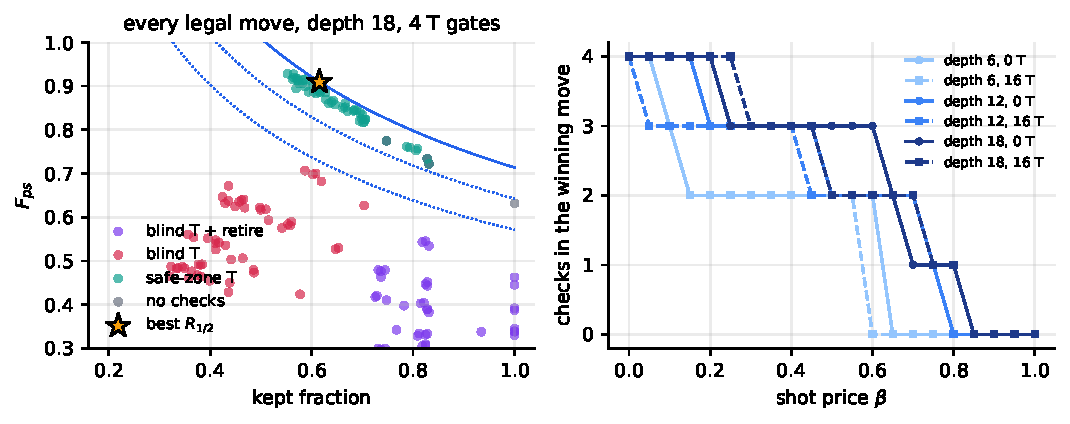
\includegraphics[width=0.92\textwidth]{fig_pareto_beta.pdf}\\
\small Deep, 4 $T$: best move \BestDeepTFourTargets{} with \BestDeepTFourPolicy{} placement, $F_0=\BestDeepTFourFzero\to F_{ps}=\BestDeepTFourFps$ at $\kappa=\BestDeepTFourKeep$, gain $\times\BestDeepTFourGain$.
\end{frame}

\begin{frame}{Can you trust the numbers?}
\begin{columns}[c]
\column{0.6\textwidth}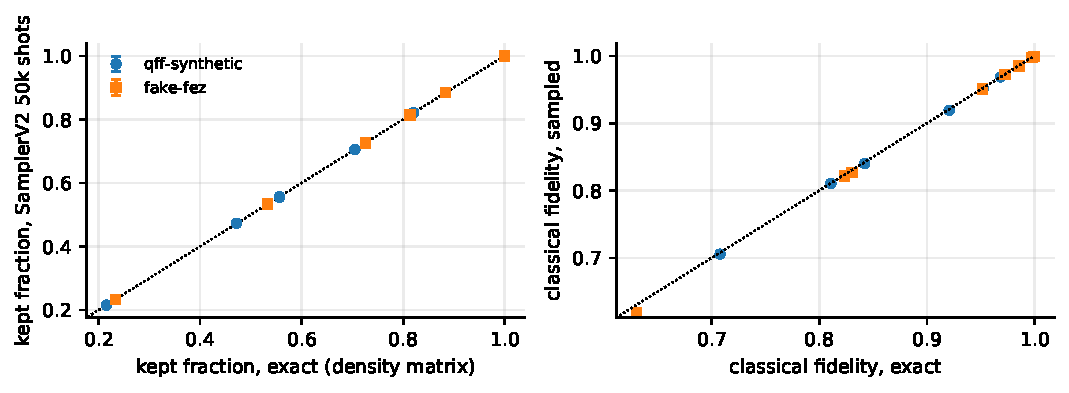
\includegraphics[width=\textwidth]{fig_validation.pdf}
\column{0.4\textwidth}\small
\begin{itemize}
  \item Exact density matrix vs.\ \texttt{SamplerV2}, 50k shots, 20 configurations: max deviation \ValKeepSigma$\sigma$ in kept fraction.
  \item Stabilizer-group identity equals statevector overlap.
  \item Noiseless runs: valid checks never fire.
  \item Five random payloads, two noise models.
\end{itemize}
\end{columns}
\end{frame}

\begin{frame}{Qiskit inside}
\begin{itemize}\setlength\itemsep{6pt}
  \item \texttt{qiskit-paulice}: \texttt{add\_pauli\_checks}, \texttt{NoiseModel}, \texttt{NoiseModel.from\_backend(FakeFez)}, \texttt{get\_postselection\_method}, \texttt{uncovered\_paulis}.
  \item \texttt{qiskit.quantum\_info}: \texttt{StabilizerState}, \texttt{Clifford}, \texttt{Statevector}, \texttt{hellinger\_fidelity}.
  \item Qiskit Aer: density-matrix simulator, \texttt{SamplerV2} primitive, GPU switch.
  \item Reproducible notebook, tests in CI, one-command rebuild, Slurm scripts.
\end{itemize}
\end{frame}

\begin{frame}{Honest limitations}
\begin{itemize}\setlength\itemsep{6pt}
  \item 6 data qubits and $\le$ 4 checks so every move is exact. Larger circuits may differ.
  \item Uniform Pauli noise, no idling noise (as in the current check picker).
  \item Coherent syndrome parity in simulation (identical statistics to classical XOR).
  \item Web game plays back pre-computed Qiskit results; live play via \texttt{sentinels play}.
\end{itemize}
\end{frame}

\begin{frame}
\centering
{\Large\bfseries Protection and magic compete for the same spacetime.}\\[14pt]
Play it: \texttt{https://Sumitchongder.github.io/spacetime-sentinels}\\[6pt]
\small Code, report and data: \texttt{github.com/Sumitchongder/spacetime-sentinels}
\end{frame}

\end{document}
